\documentclass{beamer}
\usepackage{beamerthemesplit} 
\usepackage[utf8]{inputenc}
\usepackage{default}
\usepackage{graphicx}
\usepackage{float}
\usepackage{color, colortbl}
\usepackage{xcolor}
\usepackage{caption}
\usepackage{subcaption}
\usepackage{threeparttable}
\usepackage{amsmath}


\title{Localization Procedure}
	\subtitle{Orchestrating position estimation protocols in randomly deployed WSNs}
\author[Sanabria-Russo. L, Cano. C, Bellalta. B.]{Luis Sanabria-Russo, Cristina Cano, Boris Bellalta}
\institute[UPF]{Universitat Pompeu Fabra\\
				NeTS Research Group\\
				Barcelona, Spain}
\date{\today}



\begin{document}
%------------------Title Page---------------------%
\frame{\titlepage}

\frame{\frametitle{Table of contents}\tableofcontents}

\section{Introduction}\label{intro}
\frame{\frametitle{What are Randomly Deployed WSNs?}
	\begin{itemize}
		\item Nodes are placed randomly over a field.
		\item It also encompasses deployments made at convenience.
	\end{itemize}
	
	\begin{figure}[htbp]
		\centering
		\begin{subfigure}{.5\textwidth}
			\centering
			\includegraphics[width=0.565\linewidth, angle=-90]{figures/topology.eps}
			\caption{\tiny Example random deployment of nodes
			\label{fig:topology}}
			\end{subfigure}%
		\begin{subfigure}{.5\textwidth}
			\centering
			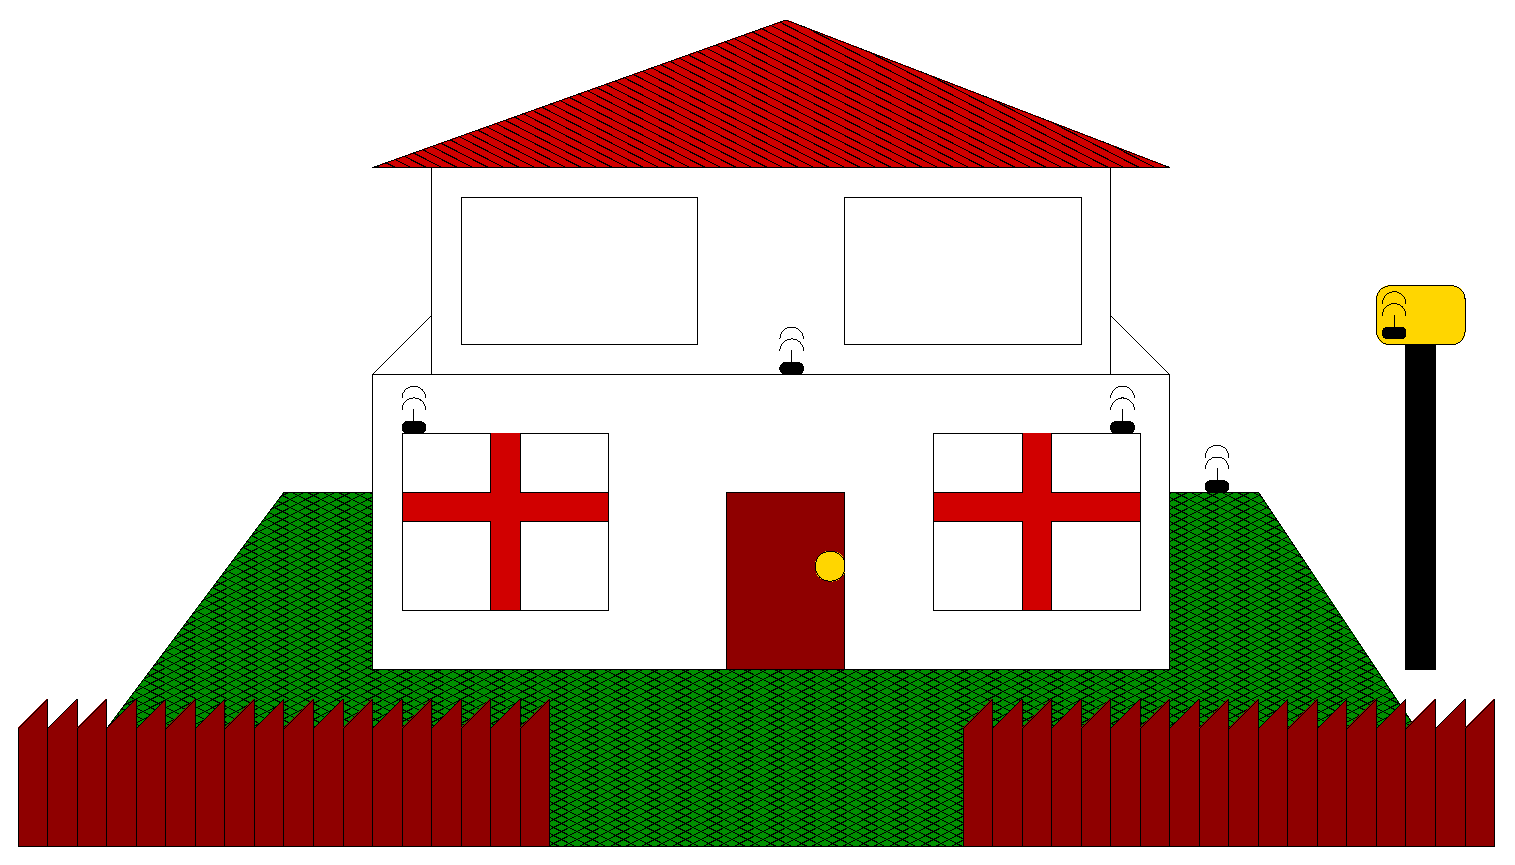
\includegraphics[width=\linewidth]{figures/house.eps}
			\caption{\tiny Example home surveillance deployment
			\label{fig:house}}
			\end{subfigure}
%	\caption{}
	\end{figure}
}


	\subsection{Characteristics}
	\frame{\frametitle{Characteristics}
		\begin{itemize}
			\item Nodes determine the best route to the sink.
			\item Ofter are easier to deploy.
			\item In case of a battery run-out, nodes can be replaced.
		\end{itemize}
		
		\begin{figure}
			\centering
			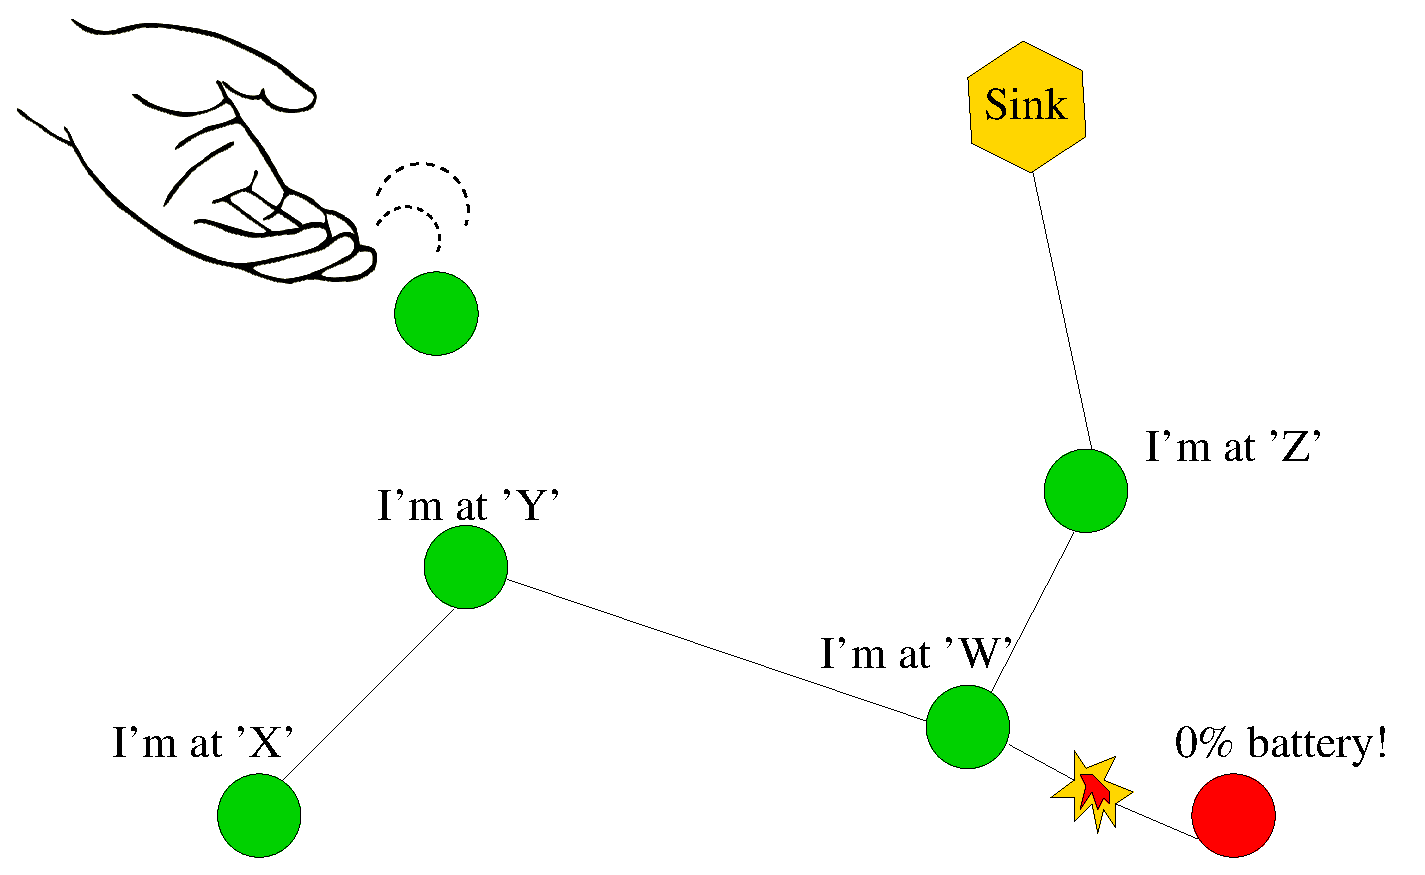
\includegraphics[width=0.565\linewidth]{figures/replacement.eps}
			\caption{\tiny Replacing nodes
			\label{fig:replacement}}
		\end{figure}%
	}

	
	\subsection{Applications}
	\frame{\frametitle{Applications}
		Because of their ease of deployment, are often used for:
			\begin{itemize}
				\item Volcano activity monitoring.
				\begin{itemize}
					\item Very dangerous or difficult places for deployment.
				\end{itemize}
				\item Forest fire detection.
				\begin{itemize}
					\item Very big areas.
				\end{itemize}
			\end{itemize}
		\begin{figure}
			\centering
			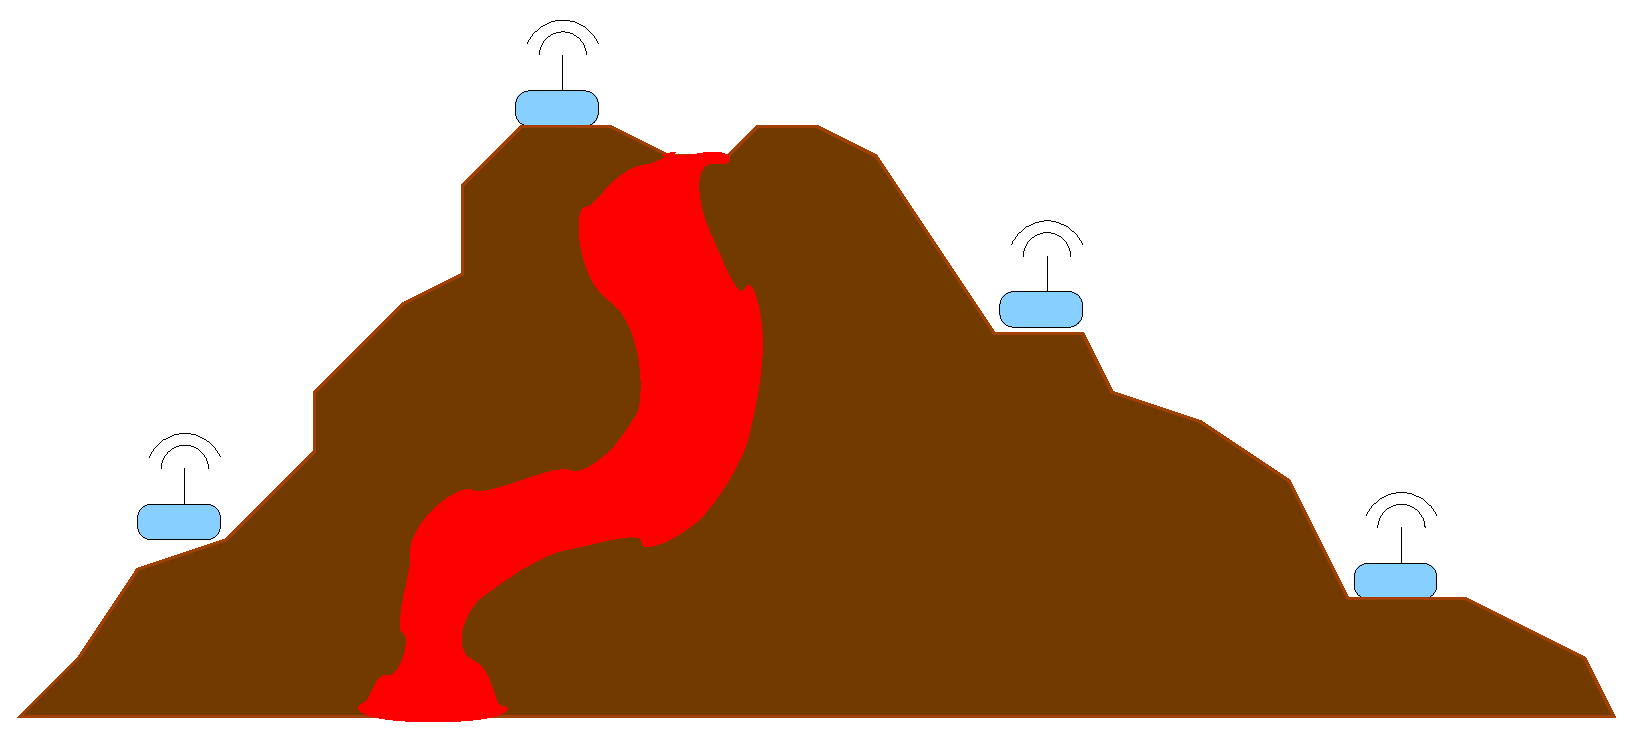
\includegraphics[width=0.565\linewidth]{figures/volcano.eps}
			\caption{\tiny Volcano monitoring example
			\label{fig:volcano}}
		\end{figure}%
	}
	
	\subsection{Pro's and Con's}
	\frame{\frametitle{Pro's and Con's of random deployments}
	Pro's:
	\begin{itemize}
		\item Allows rapid deployment.
		\item Reach very restrictive or dangerous places.
		\item Allows fast network reinforcement.
	\end{itemize}
	
	Con's:
	\begin{itemize}
		\item It is difficult to trace the metrics.
		\item Position of the nodes is not know a priori.
		\item Localization often decreases network lifetime.
	\end{itemize}
	}
	
\section{Node Localization}
\frame{\frametitle{Node Localization}
	To make metrics traceable:
	\begin{enumerate}
		\item All nodes are equipped with GPS modules.
		\begin{enumerate}
			\item Decreasing network lifetime due to the modules~$\color{red}\downarrow$.
			\item Increasing the size and weight of the nodes~$\color{red}\downarrow$.
			\item Augmenting the required budget~$\color{red}\downarrow$.
			\item Very low estimation error~$\color{green}\uparrow$.
		\end{enumerate}
		\item Some nodes use GPS modules
		\begin{enumerate}
			\item Nodes derive a position estimation from Anchors: increased estimation error~$\color{red}\downarrow$.
			\item Additional workload is added to the nodes (estimation)~$\color{red}\downarrow$.
			\item Added network traffic (\emph{Beacons}) containing location information~$\color{red}\downarrow$.
			\item Cheaper and scalable approach~$\color{green}\uparrow$.
		\end{enumerate}
	\end{enumerate}
}

	\subsection{Estimating Position by Reference}
	\frame{\frametitle{Estimating Position by Reference}
		\begin{itemize}
			\item Any \emph{Unknown} node (unaware of its position) may derive an estimation from Beacons.
			\item Beacons packets contain the position of the sender.
		\end{itemize}
		\begin{figure}[htbp]
			\centering
			\begin{subfigure}{.5\textwidth}
				\centering
				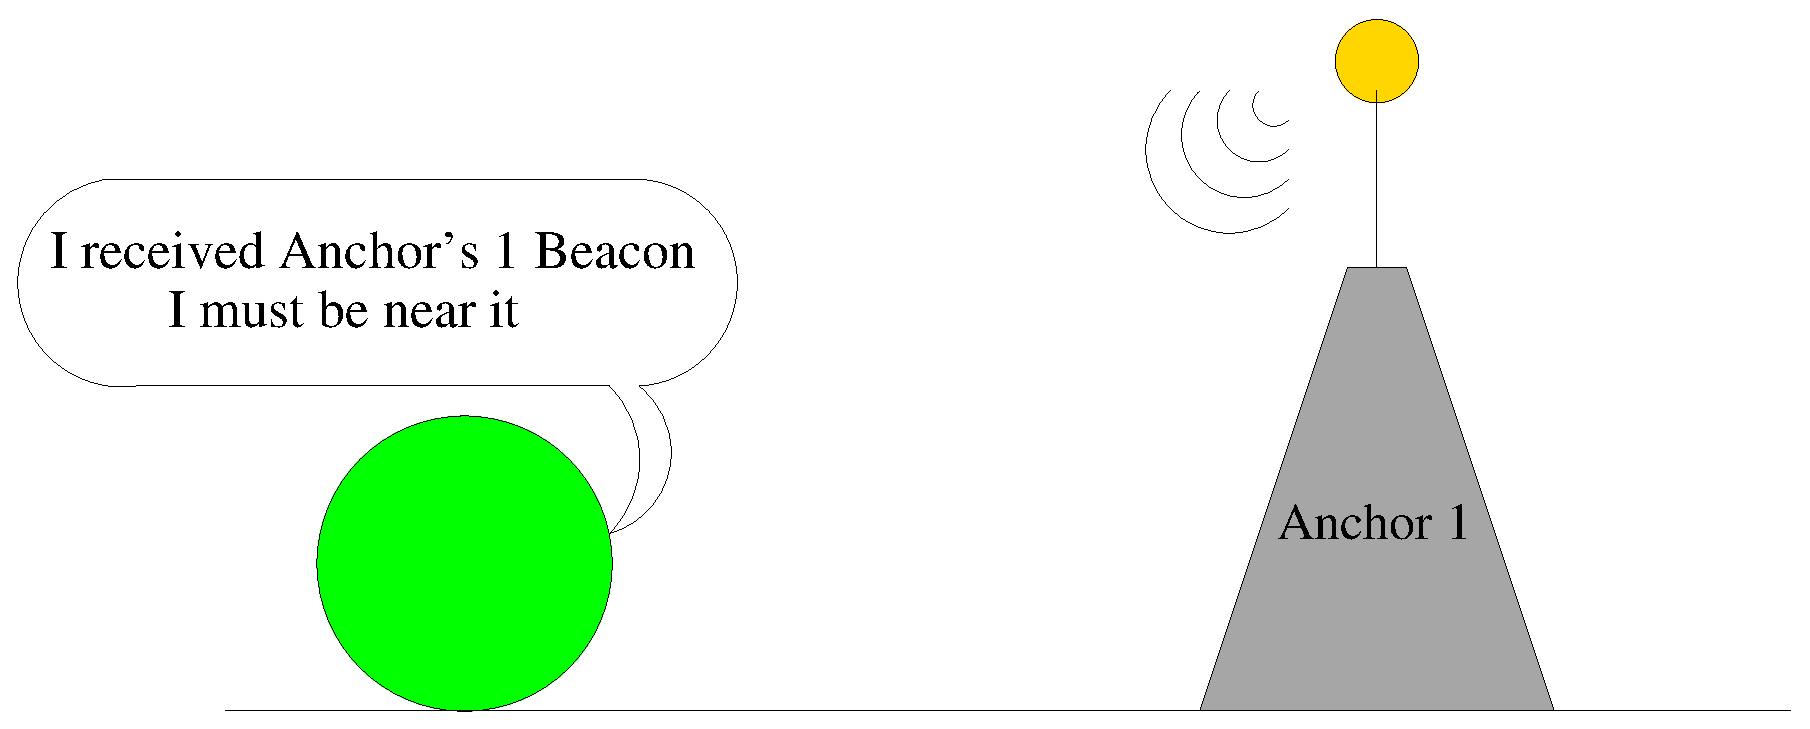
\includegraphics[width=\linewidth]{figures/coverage1.eps}
				\caption{\tiny Estimating a position with 1 Beacon
				\label{fig:coverage1}}
			\end{subfigure}%
			\begin{subfigure}{.5\textwidth}
				\centering
				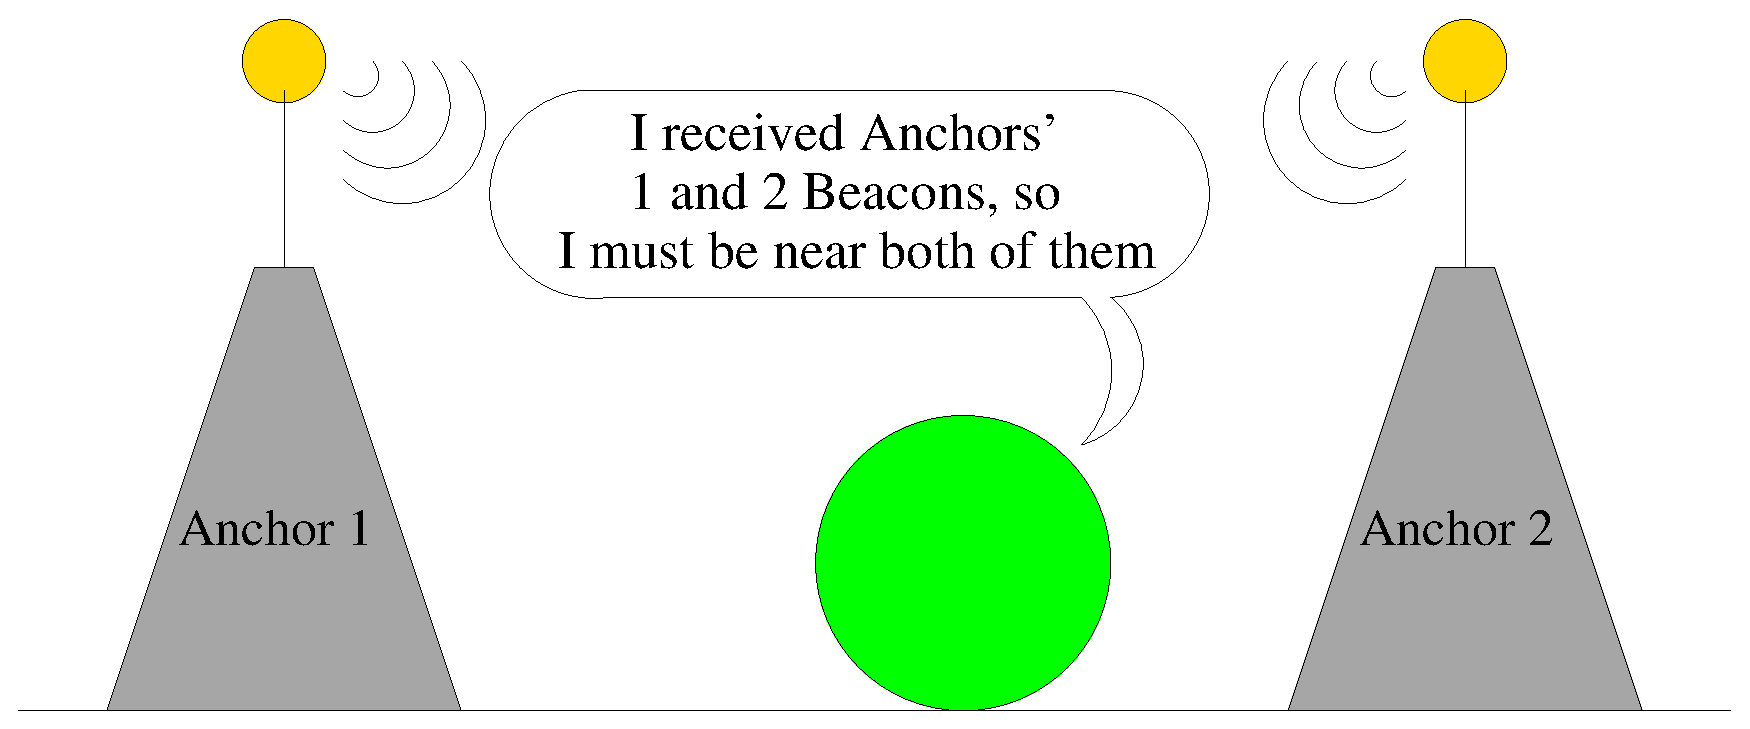
\includegraphics[width=0.97\linewidth]{figures/coverage2.eps}
				\caption{\tiny Estimating a position with 2 Beacons
				\label{fig:converage2}}
			\end{subfigure}
		%	\caption{}
		\end{figure}
		\begin{itemize}
			\item Applications may tolerate different levels of estimation errors.
		\end{itemize}
	}
	
	\frame{\frametitle{Making Range Estimations}
		\begin{itemize}
		 \item Use the propagation characteristics of Beacons
		 \begin{itemize}
			\item  Derive a straight line estimation to the transmitter.
		 \end{itemize}

		\end{itemize}
		\begin{figure}[htbp]
			\centering
			\begin{subfigure}{.5\textwidth}
				\centering
				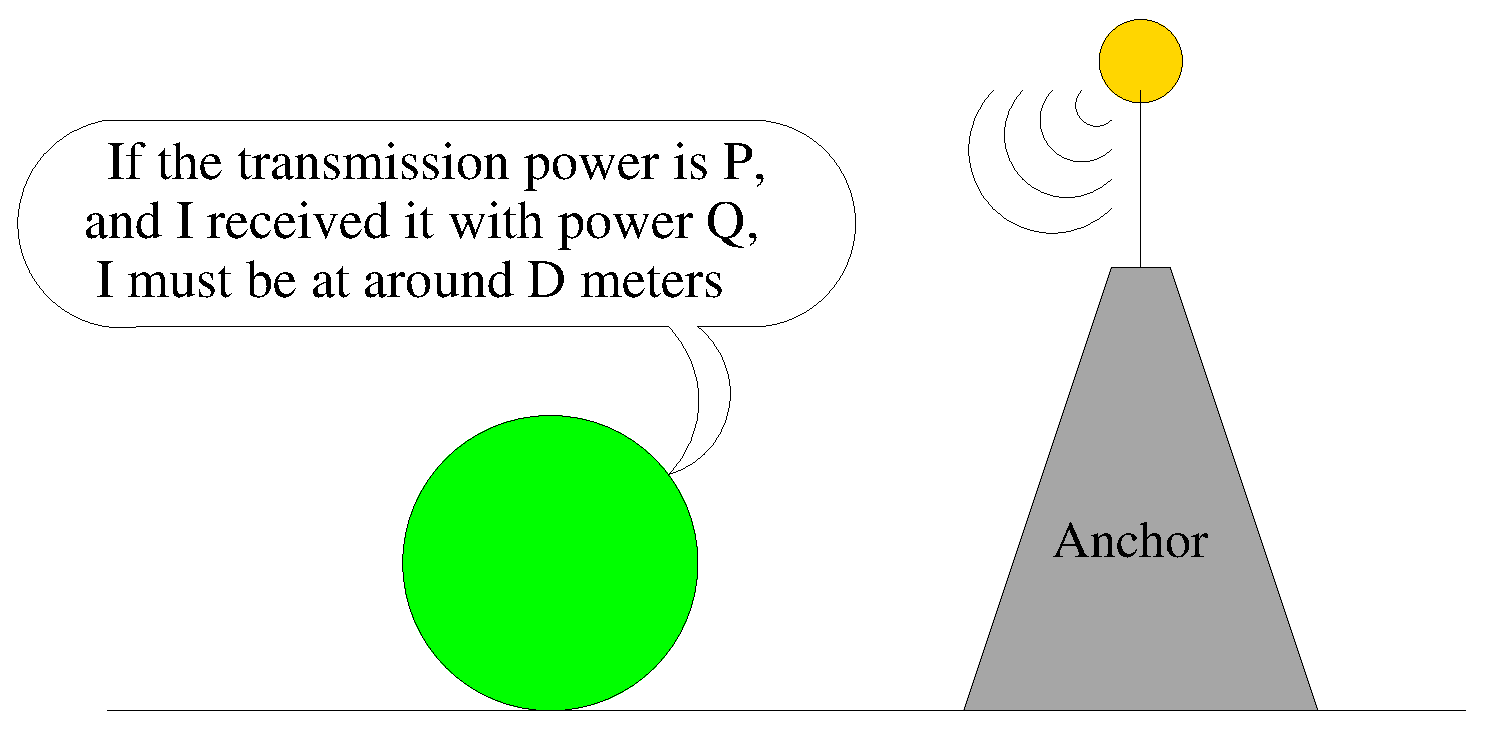
\includegraphics[width=\linewidth]{figures/RSSI.eps}
				\caption{\tiny RSSI position estimation
				\label{fig:RSSI}}
			\end{subfigure}%
			\begin{subfigure}{.5\textwidth}
				\centering
				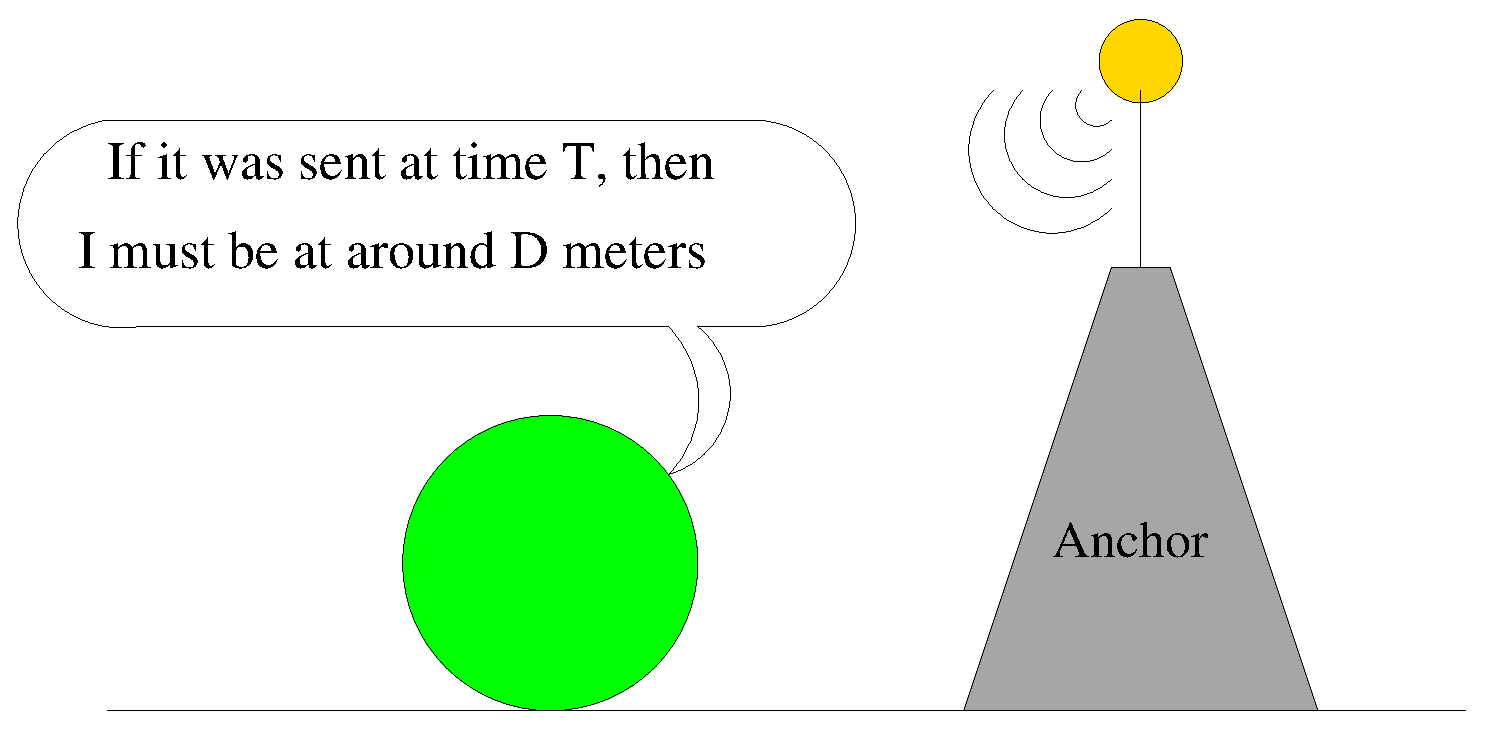
\includegraphics[width=\linewidth]{figures/ToA.eps}
				\caption{\tiny Time of Arrival (ToA)
				\label{fig:ToA}}
			\end{subfigure}
		%	\caption{}
		\end{figure}
	}
	
	
	\subsection{Localization Protocols}
	\frame{\frametitle{Localization Protocols}
		%In \emph{Anchor-based} deployments, position estimation protocols are often divided in:\\
		\begin{minipage}[l]{0.5\textwidth}
			{\bfseries ~~~~~~~~~~~~~Range-free}
			\begin{figure}
				\centering
				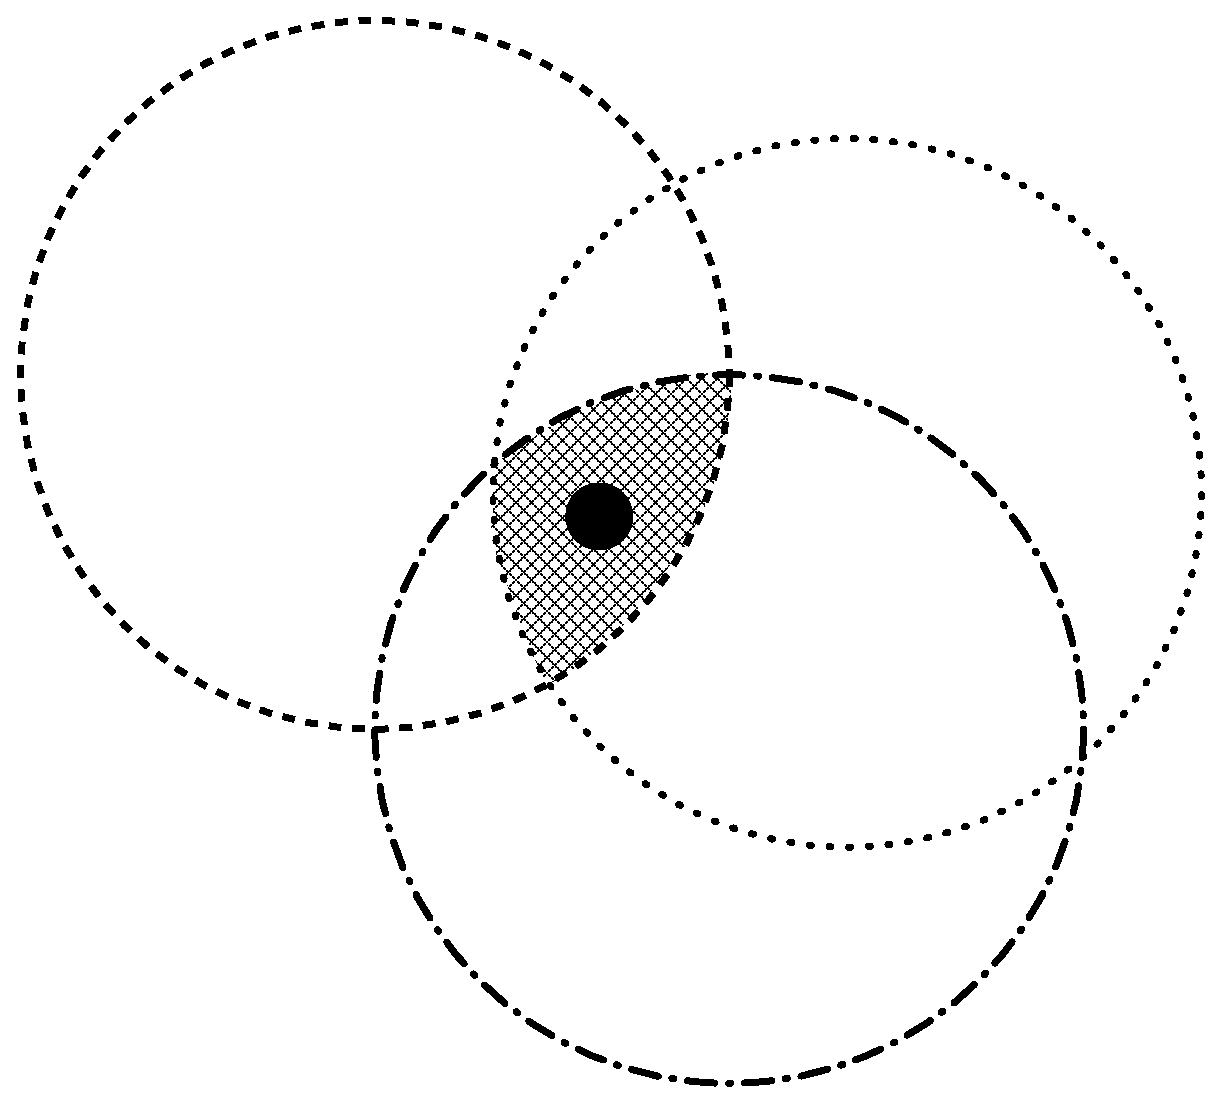
\includegraphics[width=0.75\linewidth]{figures/bounding_box.eps}
				\caption{\small Bounding-Box example
				\label{fig:bounding-box}}
			\end{figure}%

		\end{minipage}%
		\hfill
		\begin{minipage}[r]{0.5\textwidth}
			{\bfseries ~~~~~~~~~~Range-based}
			\begin{figure}
				\centering
				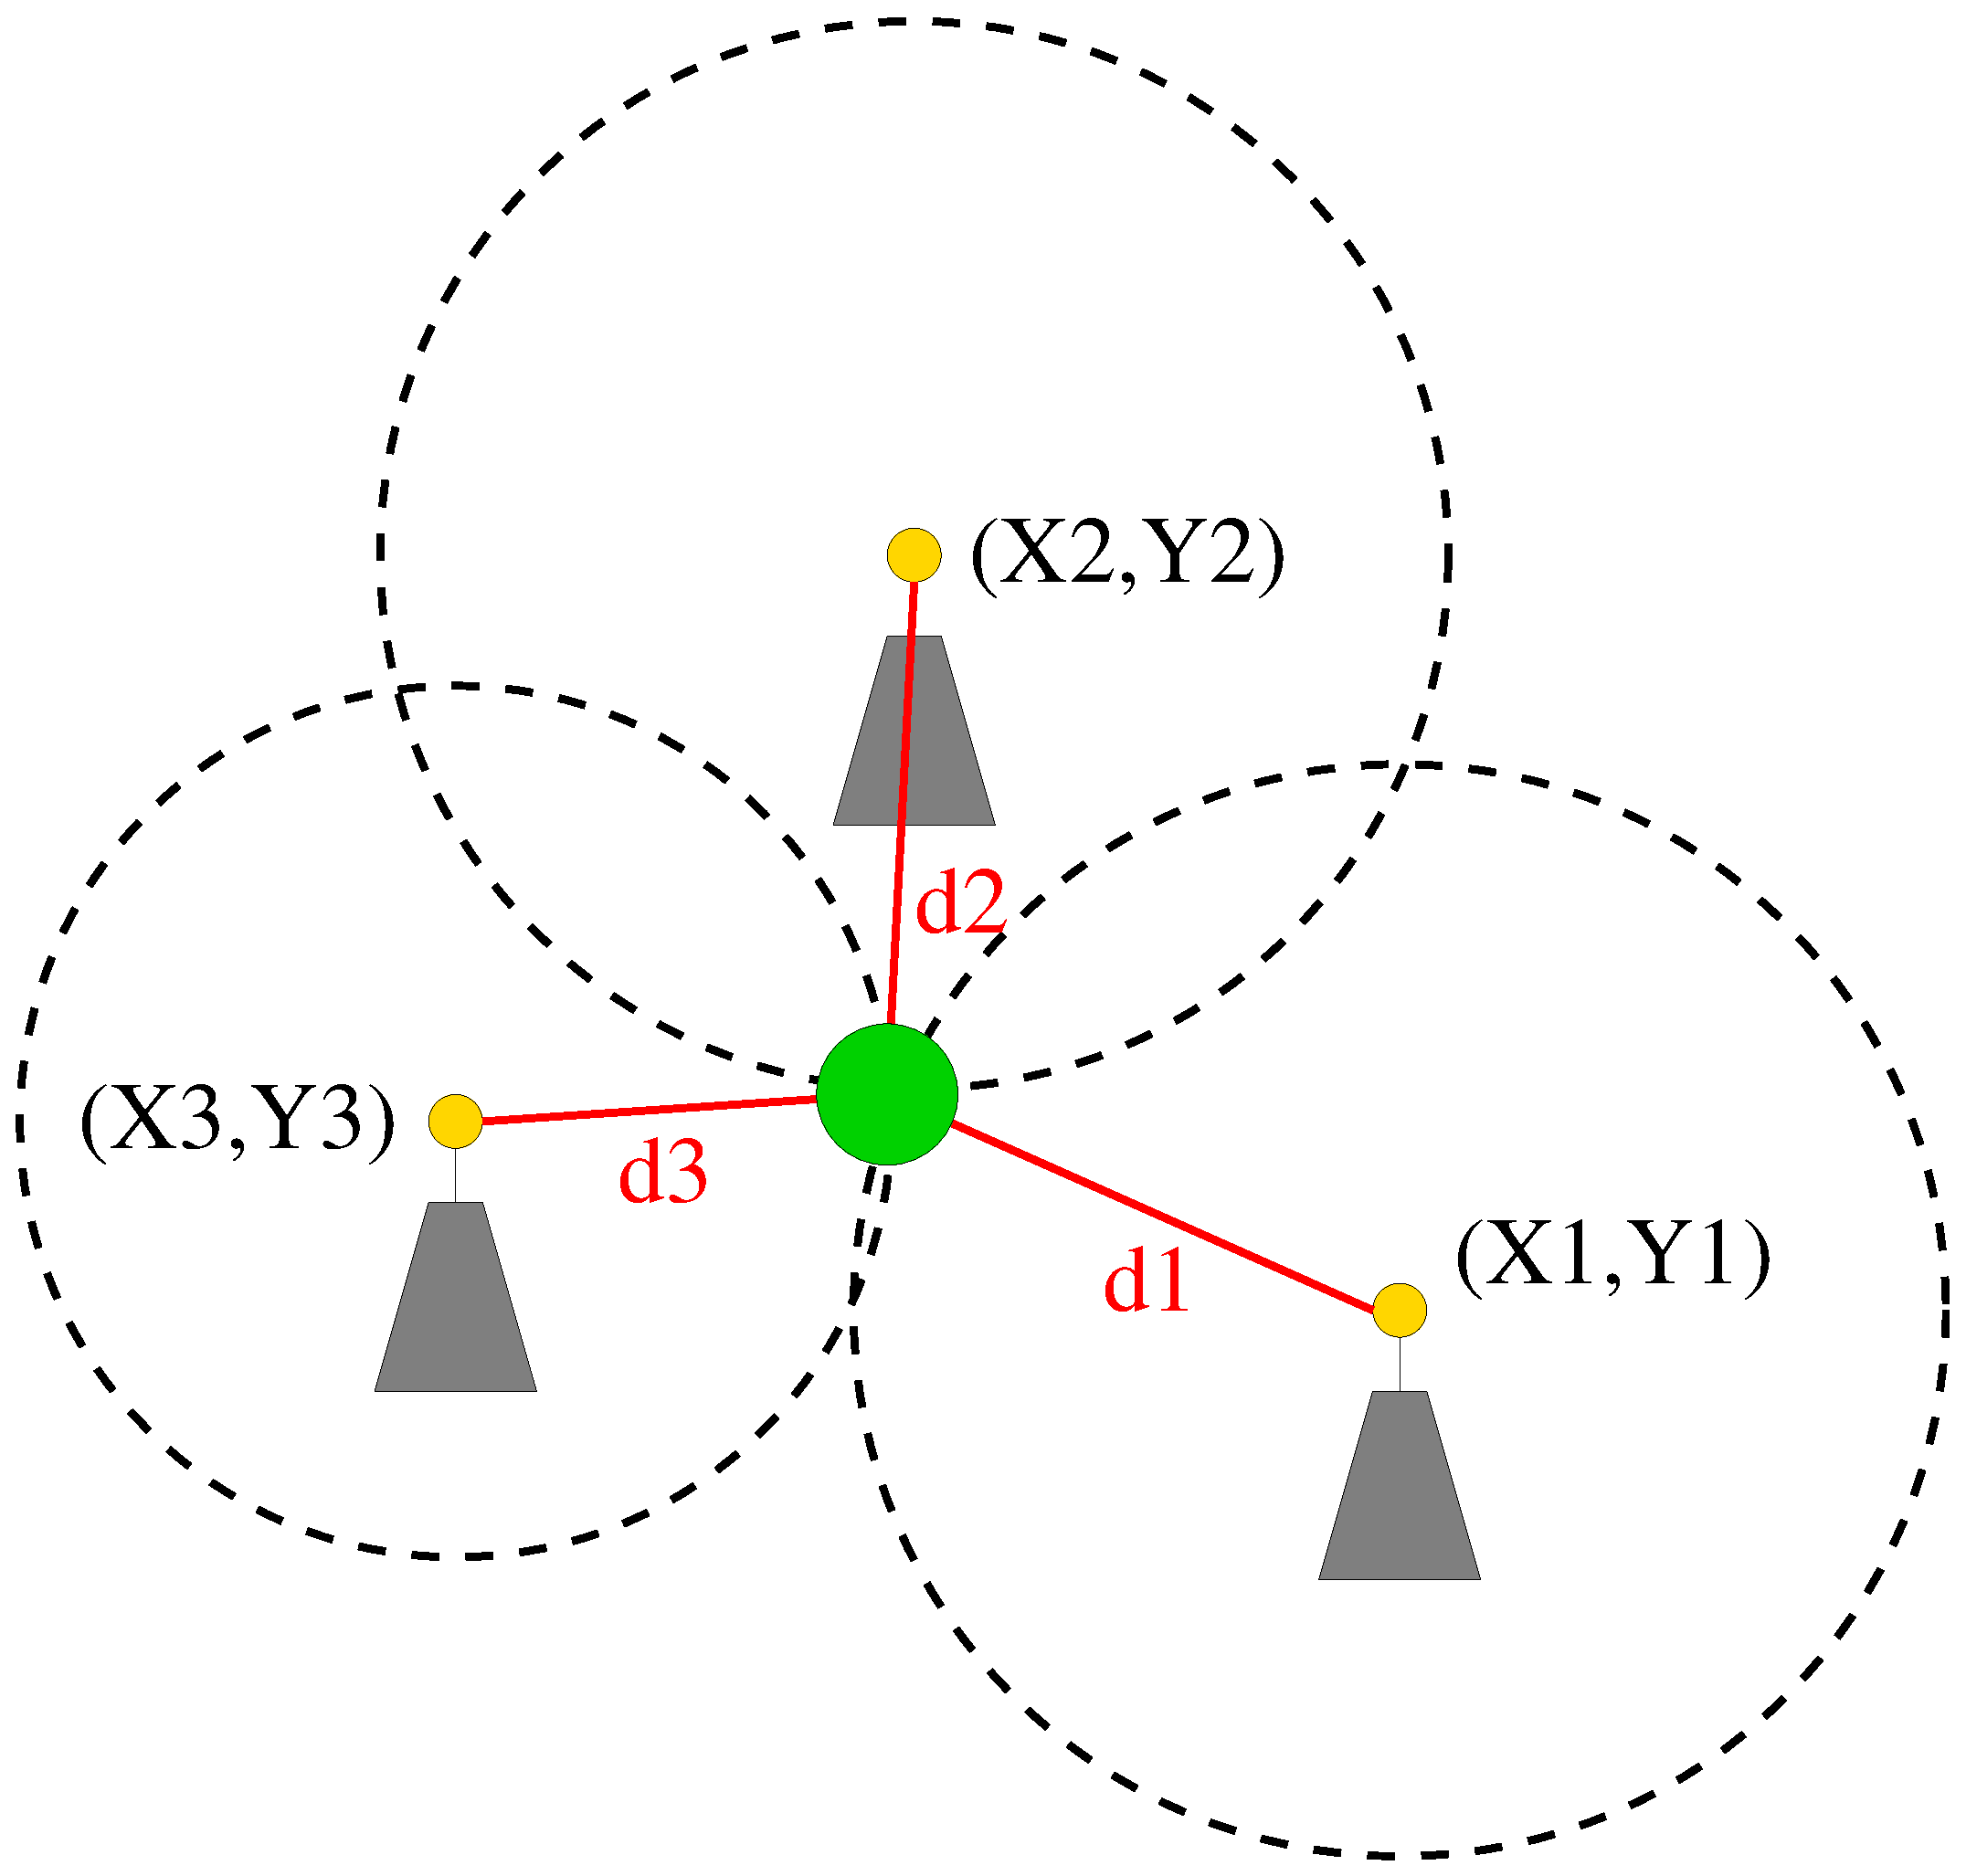
\includegraphics[width=0.7\linewidth]{figures/lateration.eps}
				\caption{\small Lateration example
				\label{fig:lateration}}
			\end{figure}%
% 			\begin{itemize}
% 				\item Also uses ranging techniques to add constraints.
% 			\end{itemize}

		\end{minipage}%
	}
	
	\frame{\frametitle{Range-free and Range-based}
		Range-free protocols:
		\begin{itemize}
 			\item Only consider the effective connection with Anchors.
 			\item Usually consume less battery.
 			\item Error is subject to the number of connections to Anchors.
		\end{itemize}
		Range-based protocols:
		\begin{itemize}
			\item Use ranging techniques to constrain the estimation.
			\item Increased battery consumption related to the ranging technique.
			\item Error is usually reduced due to the availability of more data.
		\end{itemize}

	}
	
	\frame{\frametitle{Locating Nodes}
		\begin{itemize}
			\item Applications dictate the maximum estimation error.
			%\begin{itemize}
%				\item Can be coarse (meters) or strict (centimeters).
%			\end{itemize}
			\item Protocol performance is limited by the network-{\bfseries environmanetal conditions} surrounding each node:
			\begin{itemize}
				\item $\#$ of surrounding Anchors.
				\item Network delay.
				\item Available throughput.
				\item Processing capabilities.
			\end{itemize}
			\item {\bfseries Deployments} may have different {\bfseries considerations} regarding:
			\begin{itemize}
				\item Network lifetime.
				\item Location accuracy.
				\item Traffic overhead.
				\item Convergence time.
			\end{itemize}
		\end{itemize}

	One protocol cannot perform well in all possible scenarios	
	}
	
	\subsection{Composability of Localization Protocols}
	\frame{\frametitle{Composability}
		\begin{itemize}
			\item Combines different protocols to achieve better results.
			\begin{figure}
				\centering
				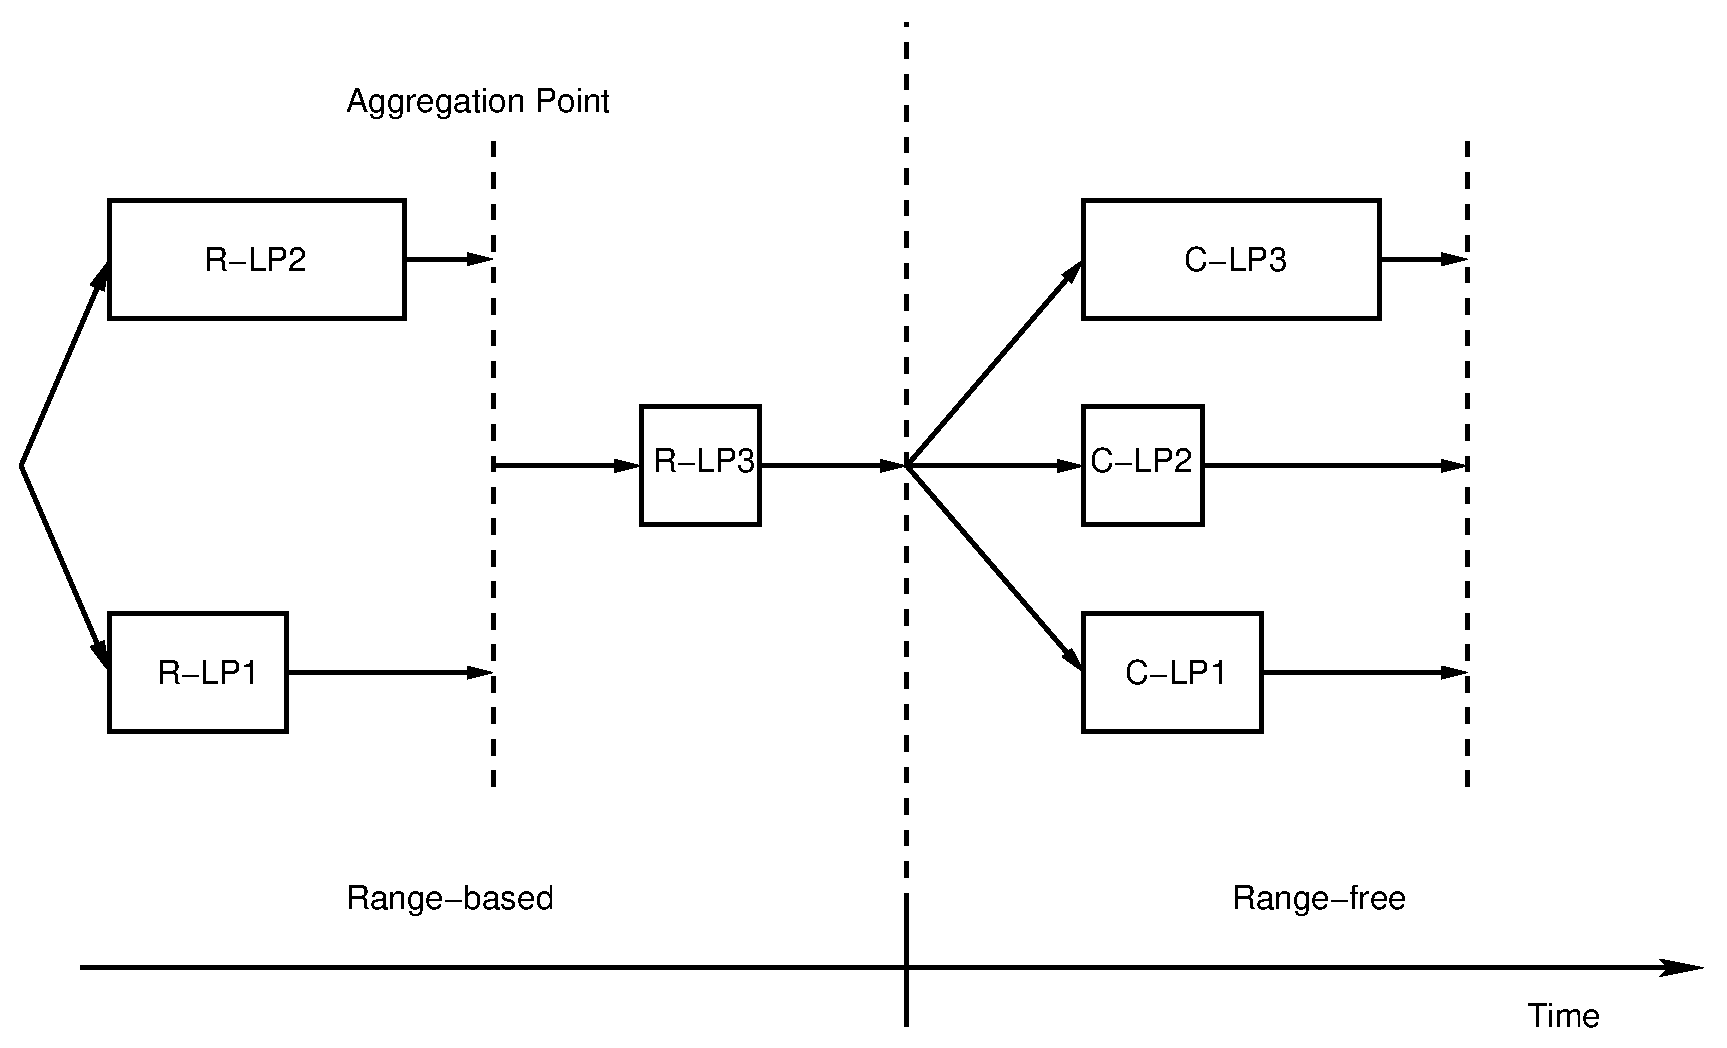
\includegraphics[width=0.7\linewidth]{figures/composability.eps}
				\caption{\small Composability\tiny{\footnote{\tiny{Redrawn from Stoleru, R., Stankovic, J., Son, S.H., “On Composability of Localization Protocols for Wireless Sensor Networks,” Network, IEEE, vol. 22, no. 4, pp. 21–25, 2008.}}}
				\label{fig:composability}}
			\end{figure}
		\end{itemize}
	}
	
	\frame{\frametitle{Composability}
		\begin{itemize}
			\item Leverages weaknesses of some protocols with strengths of others.
			\item Protocols are executed sequentially according to accuracy thresholds.
			\item Brings some questions:
			\begin{itemize}
				\item How are protocols selected?
				\item How are thresholds set?
				\item Is it static-sequential execution the way to go?
			\end{itemize}
		\end{itemize}
	}
	
\section{Localization Procedure}
\subsection{Definitions}
\frame{\frametitle{Localization Procedure}
Is based on:
	\begin{itemize}
		\item Protocol's performance is dependent on the environmental conditions.
		\item Selected protocols must comply with the deployment considerations.
	\end{itemize}
The Localization Procedure:
	\begin{itemize}
		\item Analyzes the node's environmental conditions.
		\item Identifies a suitable set of protocols.
	\end{itemize}
}

\frame{\frametitle{Localization Procedure}
\begin{figure}
		\centering
		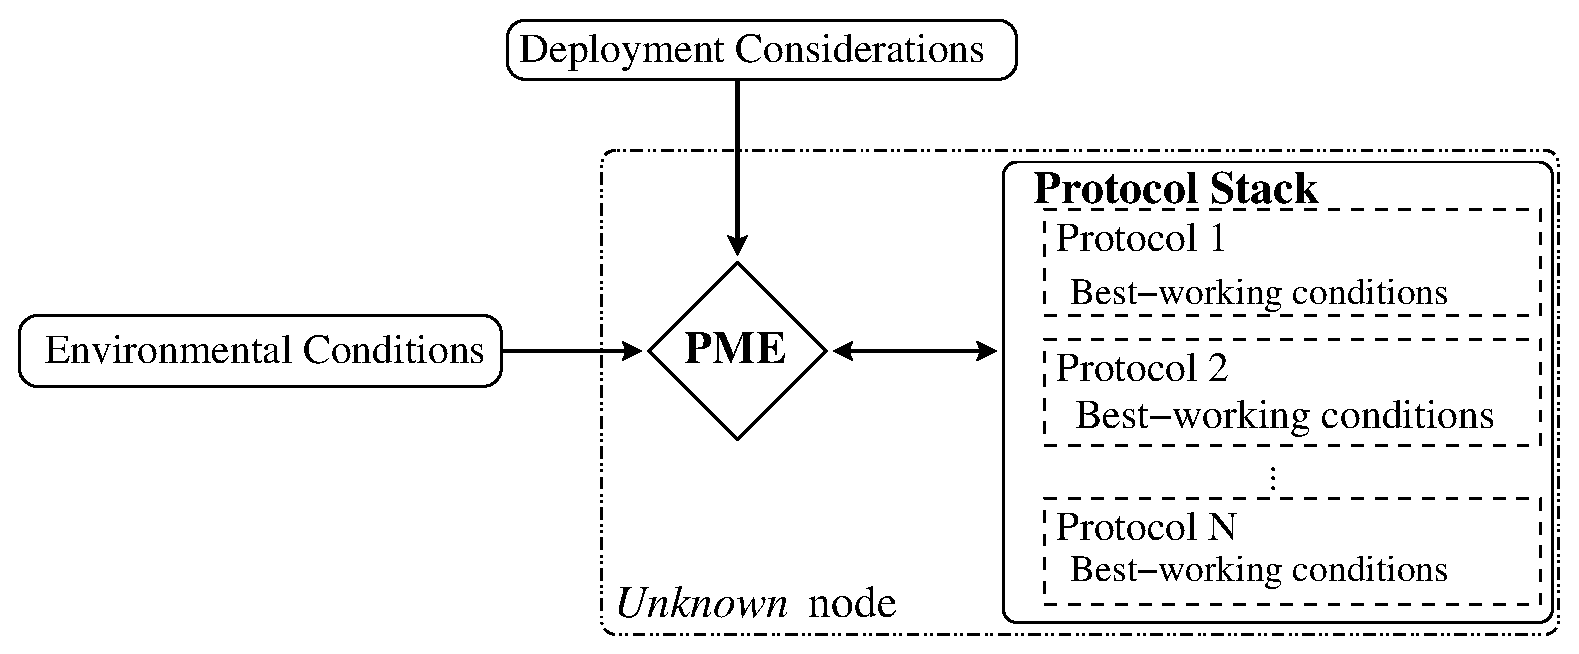
\includegraphics[width=0.9\linewidth]{figures/LocProc.eps}
		\caption{\small Localization Procedure
		\label{fig:LocProc}}
\end{figure}
}

\subsection{Pattern Matching Engine}
\frame{\frametitle{Localizatitheon Procedure}
	The Pattern Matching Engine (PME):
	\begin{itemize}
		\item Manages the execution of \emph{characterized}{\tiny{\footnote{\tiny{Their best-working conditions are known.}}}} localization protocols.
		\item Selects a set of protocols based on the environmental conditions.
		\item Reorders the execution based on the deployment considerations.
	\end{itemize}
}

\subsection{Evaluation}
\frame{\frametitle{Evaluation tools}

\begin{itemize}
	\item Bounding-Box and Lateration are tested.
	\begin{itemize}
		\item Popular.
		\item Some of their best-working conditions are known.
		\item Range-free and range-based example.
		\item $100$~m~x~$100$~m flat surface.
	\end{itemize}
\end{itemize}

\begin{table}[htbp]
  \centering
  \begin{threeparttable}[htbp]
    \begin{tabular}{c||c||c}
    \hline
    \bfseries Characteristic & \bfseries Lateration & \bfseries Bounding-Box\\
    \hline\hline 
    Env. Conditions & At least 4 \emph{Anchors} & At least 1 \emph{Anchor}\\
    Accuracy & 2-10 meters & Coarse{\tiny \footnote{Location area upper-bounded by \emph{Anchor}'s radio range (R).}}\\
    Energy Consumption & Low & Very low{\tiny\footnote{Can be treated as a discrete problem.}}\\
    \hline
    \end{tabular}
  \end{threeparttable}
\end{table}
}


\frame{\frametitle{Evaluation tools}

\begin{itemize}
	\item Modified version of the SENSE simulator{\tiny{\footnote{\tiny{Chen, G., Branch, J., Pflug, M., Zhu, L., Szymanski, B., “SENSE: a wireless sensor network simulator,” Advances in Pervasive Computing and Networking, pp. 249–267, 2005.}}}}
	\item Deployment considerations: high accuracy and long network lifetime.
	\item Two channel models: free space and shadowing.
\end{itemize}
\begin{figure}
		\centering
		\includegraphics[width=0.35\linewidth,angle=-90]{figures/avgBeaconPerNode.eps}
\end{figure}

}

\frame{\frametitle{Battery Consumption}
\begin{itemize}
	\item Similar battery consumption.
\end{itemize}
\begin{figure}[htbp]
		\centering
		\begin{subfigure}{.5\textwidth}
			\centering
			\includegraphics[width=0.7\linewidth, angle=-90]{figures/battery.eps}
			\caption{\tiny Individual execution
			\label{fig:individual}}
			\end{subfigure}%
		\begin{subfigure}{.5\textwidth}
			\centering
			\includegraphics[width=0.7\linewidth,angle=-90]{figures/pmeBat.eps}
			\caption{\tiny Localization Procedure
			\label{fig:LocProc-Bat}}
			\end{subfigure}
%	\caption{}
\end{figure}
}


\frame{\frametitle{Located Nodes}
\begin{itemize}
	\item Increased number of located nodes.
\end{itemize}
\begin{figure}[htbp]
		\centering
		\begin{subfigure}{.5\textwidth}
			\centering
			\includegraphics[width=0.7\linewidth, angle=-90]{figures/locatedNodes.eps}
			\caption{\tiny Individual execution}
			\end{subfigure}%
		\begin{subfigure}{.5\textwidth}
			\centering
			\includegraphics[width=0.7\linewidth,angle=-90]{figures/pmeLocNodes.eps}
			\caption{\tiny Localization Procedure}
			\end{subfigure}
%	\caption{}
\end{figure}
}


\frame{\frametitle{Straigh-line Error}
\begin{itemize}
	\item Greater \emph{average} error than in Lateration-only scenarios.
\end{itemize}
\begin{figure}[htbp]
		\centering
		\begin{subfigure}{.5\textwidth}
			\centering
			\includegraphics[width=0.7\linewidth, angle=-90]{figures/error.eps}
			\caption{\tiny Individual execution}
			\end{subfigure}%
		\begin{subfigure}{.5\textwidth}
			\centering
			\includegraphics[width=0.7\linewidth,angle=-90]{figures/pmeError.eps}
			\caption{\tiny Localization Procedure}
			\end{subfigure}
%	\caption{}
\end{figure}
}

\section{Remarks}
\frame{\frametitle{Remarks}
\begin{itemize}
	\item Despite of greater error than Lateration:
	\begin{itemize}
		\item Number of located nodes is increased.
		\item In the individual execution, these nodes have infinite error.
		\item Similar battery consumption.
	\end{itemize}
	\item A carefully selected set of protocols can work on more scenarios.
	\item Allowing node-\emph{Beacoming} and location information exchange:
	\begin{itemize}
		\item Cetralized protocols.
		\item More scenarios: NLoS, anisotropic topologies.
	\end{itemize}
\end{itemize}
}
	
\end{document}














